\section{理论基础}

\subsection{时间序列}
时间序列是在一系列时间点上收集到的观测值的集合。更形式化地说,一个时间序列可以被定义为一个随机过程 $\left\{X_t\right\}$ 的一次观测实现(realization),其中 $t$ 属于某个索引集 $T$ 。在大多数应用中,索引集 $T$ 代表时间,并且通常被假定为离散且等间隔的,例如 $T=\{1,2, \ldots, N\}$ 或 $T=$ $\left\{t_1, t_2, \ldots, t_N\right\}$ ,其中 $N$ 是观测的总数。每个 $X_t$ 是在时间点 $t$ 观测到的数值。

\textbf{定义 2.1} (时间序列)\cite{shumway2000time}:
一个时间序列是一个按时间顺序索引的观测序列 $\left\{x_t: t \in T\right\}$ ,其中 $x_t$ 是在时间点 $t$ 记录的观测值,而 $T$ 是一个有序的时间索引集。

如果每个观测值 $x_t$ 是一个单一的数值(即 $x_t \in \mathbb{R}$ ),则该序列称为单变量时间序列(univariate time series)。如果每个观测值 $x_t$ 是一个 $k$ 维向量(即 $x_t \in \mathbb{R}^k, k>1$ ),则该序列称为多变量时间序列 (multivariate time series)。在本研究中,我们主要关注单变量时间序列。

时间序列分析的主要目标是理解这些观测序列的潜在结构和动态特性,以便进行描述、解释、预测或控制。这些序列可以来源于各种领域,如经济学(例如,股票价格)、气象学(例如,每日温度)、医学(例如,心电图信号)和工程学(例如,传感器读数)。

\subsection{点云}
在几何处理和数据分析领域,点云是描述和表示三维形状或高维数据对象的一种基本形式。点云的定义在理论文献中通常与拓扑和几何分析相关联,它构成了从离散采样数据中推断连续结构的基础。

\textbf{定义 2.2} (点云)\cite{dey2022computational}:
一个点云 $P$ 是在某个度量空间 $\left(M, d_M\right)$ 中的一个有限点集,通常我们考虑的是 $m$ 维欧几里得空间 $\mathbb{R}^m$ 及其标准欧几里得距离。因此,一个点云可以表示为 $P=\left\{p_1, p_2, \ldots, p_k\right\} \subset \mathbb{R}^m$ ,其中每个 $p_i$ 是一个 $m$ 维向量,代表空间中的一个采样点。

从计算拓扑的角度来看,点云通常被视为从某个未知的、潜在的几何对象或数据分布中采样得到的结果。拓扑数据分析(TDA)的核心任务之一便是从这些离散的点云数据中推断出该潜在对象的拓扑不变量和几何特征。点云本身不包含点与点之间的连接信息,但其空间分布蕴含了原始形状的结构。后续的拓扑分析方法,如构建单纯复形(例如 Vietoris-Rips 复形或 Čech复形),正是基于点云中点之间的邻近关系来显式地构建这些连接,从而揭示数据的"形状"。

在本研究中,时间序列数据将通过特定的嵌入技术(详见第3章)转换为高维欧几里得空间中的点云,这些点云随后将作为持续同调分析的输入,以提取其拓扑特征用于分类任务。
% 海彤的参考文献引用 1021736289.nh

\subsection{持续同调的基本概念}
\subsubsection{滑动窗口}
为细致考察时间序列的局部拓扑动态,本研究采用滑动窗口技术,避免了对整个序列进行全局性比较的局限性。该技术通过将原始时间序列分割为一系列等长的连续子区间(即窗口),使得能够在每个独立的子区间上运用持久同调等拓扑数据分析工具,从而逐段提取其拓扑特征。滑动窗口的具体定义如下:

\textbf{定义 2.3}(滑动窗口)\cite{1021736289.nh} :考虑一个具有 $m$ 个通道、时间长度为 $l$ 的时间序列信号,记为 $\left\{\mathrm{x}_l^m\right\}$ 。在任意时间点 $t_n$ ,该信号在空间上可表示为一个点 $x\left(t_n\right)=$ $\left(x_n^1, x_n^2, \ldots x_n^m\right) \in \mathbb{R}^m$ 。通过滑动窗口机制从时间序列 $\left\{\mathrm{x}_l^m\right\}$ 中提取的第 $i$ 个子区间 $X_i$ 可表示为:
$$
    X_i=\left(x\left(t_{1+s(i-1)}\right), x\left(t_{2+s(i-1)}\right), \ldots x\left(t_{w+s(i-1)}\right)\right)
$$
此处,$w$ 代表滑动窗口的宽度,$s$ 代表窗口滑动的步长。
采用这种逐段分析的策略,有助于捕捉时间序列在不同阶段拓扑结构的演变,进而更精确地刻画其动态发展过程。相较于全局性的分析方法,滑动窗口技术在识别局部模式和动态变化方面展现出更佳的性能,这对于提升后续分类与预测任务的准确性具有积极意义。因此,本研究借此方法深入挖掘时间序列的局部拓扑信息,以期揭示数据中潜在的结构性规律。

\subsubsection{同伦}
在拓扑学的研究中,同伦是刻画映射之间以及拓扑空间之间 ``连续形变'' 关系的一个基本概念。它为拓扑不变量的定义和计算提供了重要的理论途径,使得我们能够对空间的几何形态进行更深层次的分类与理解。下面将依次介绍映射的同伦、道路的同伦以及空间的同伦等价等核心定义。

\textbf{定义 2.4} (映射的同伦)\cite{armstrong2013basic}:
设 $X$ 与 $Y$ 为拓扑空间,$f, g: X \to Y$ 为两个连续映射。若存在一个连续映射 $H: X \times I \to Y$,其中 $I = [0, 1]$ 表示单位闭区间,使得对于任意 $x \in X$,均满足:
\begin{enumerate}
    \item $H(x, 0) = f(x)$
    \item $H(x, 1) = g(x)$
\end{enumerate}
则称映射 $f$ 与 $g$ 是 \textbf{同伦的 (homotopic)},记为 $f \simeq g$。映射 $H$ 称为从 $f$ 到 $g$ 的一个 \textbf{同伦 (homotopy)}。

在此定义中,参数 $t \in I$ 可被视为时间。当 $t$ 从 $0$ 连续变化至 $1$ 时,映射 $H(\cdot, t): X \to Y$ 作为 $X$ 到 $Y$ 的一个连续映射族,实现了从 $f$ 到 $g$ 的连续过渡。同伦关系是 $X$ 到 $Y$ 的所有连续映射集合上的一个等价关系。

接下来,我们考虑同伦在道路这一特殊映射上的具体体现。

\textbf{定义 2.5} (道路及其(定端)同伦)\cite{armstrong2013basic}:
设 $X$ 为一拓扑空间。$X$ 中的一条 \textbf{道路 (path)} 是指一个从单位区间 $I = [0,1]$ 到 $X$ 的连续映射 $\alpha: I \to X$。称 $\alpha(0)$ 为道路 $\alpha$ 的 \textbf{起点 (initial point)},$\alpha(1)$ 为其 \textbf{终点 (terminal point)}。

设 $\alpha, \beta: I \to X$ 为两条具有相同起点 $x_0 = \alpha(0) = \beta(0)$ 和相同终点 $x_1 = \alpha(1) = \beta(1)$ 的道路。若存在一个连续映射 $H: I \times I \to X$,使得对于任意 $s, t \in I$,均满足:
\begin{enumerate}
    \item $H(s, 0) = \alpha(s)$
    \item $H(s, 1) = \beta(s)$
    \item $H(0, t) = x_0$ \quad (保持起点固定)
    \item $H(1, t) = x_1$ \quad (保持终点固定)
\end{enumerate}
则称道路 $\alpha$ 与 $\beta$ 是 \textbf{(保持端点不动的)同伦的 (homotopic relative to endpoints)},或称它们是 \textbf{定端同伦的}。映射 $H$ 称为 $\alpha$ 到 $\beta$ 的一个 \textbf{定端同伦 (homotopy of paths fixing endpoints)}。

定端同伦关系是连接固定起点 $x_0$ 和固定终点 $x_1$ 的所有道路集合上的一个等价关系。此等价关系下的等价类称为 \textbf{道路的同伦类 (homotopy class of paths)}。

最后,同伦的概念可进一步用于定义拓扑空间之间的一种更为宽泛的等价关系。

\textbf{定义 2.6} (空间的同伦等价)\cite{armstrong2013basic}:
设 $X$ 与 $Y$ 为两个拓扑空间。若存在连续映射 $f: X \to Y$ 及 $g: Y \to X$,使得复合映射 $g \circ f: X \to X$ 同伦于 $X$ 上的恒同映射 $id_X$ (即 $g \circ f \simeq id_X$),并且复合映射 $f \circ g: Y \to Y$ 同伦于 $Y$ 上的恒同映射 $id_Y$ (即 $f \circ g \simeq id_Y$),则称拓扑空间 $X$ 与 $Y$ 是 \textbf{同伦等价的 (homotopy equivalent)},或者称它们具有相同的 \textbf{同伦型 (homotopy type)},记为 $X \simeq Y$。此时,映射 $f$ (或 $g$) 称为一个 \textbf{同伦等价映射 (homotopy equivalence)}。

若一个拓扑空间 $X$ 同伦等价于一个单点空间 $\{*\}$,则称 $X$ 为 \textbf{可缩空间 (contractible space)}。这意味着 $X$ 可以在自身内部连续地收缩到一个点。

同伦理论是代数拓扑学的重要组成部分,它通过研究空间的形变性质来揭示其深层的拓扑结构。虽然本研究主要聚焦于持续同调,同伦理论所蕴含的关于形状稳定性和连续变形的思想,为理解拓扑数据分析的本质提供了有益的视角。

\subsubsection{单纯形与单纯复形}
% 这里补充定义
为了从离散的点云数据中提取拓扑信息,拓扑数据分析(TDA)通常首先将点云转化为一种组合结构,即单纯复形。单纯复形由更基本的单元——单纯形——构成。

\textbf{定义 2.7} (仿射无关与凸包)\cite{zomorodian2004computing}:
设 $v_0, v_1, \ldots, v_k$ 是欧几里得空间 $\mathbb{R}^m$ 中的一组点。如果向量 $v_1-v_0, v_2-v_0, \ldots, v_k-v_0$ 是线性无关的,则称这些点是 \textbf{仿射无关的 (affinely independent)}。
这组点 $V = \{v_0, v_1, \ldots, v_k\}$ 的 \textbf{凸包 (convex hull)},记为 $\text{conv}(V)$,是指所有形如 $\sum_{i=0}^k \lambda_i v_i$ 的点的集合,其中 $\lambda_i \ge 0$ 且 $\sum_{i=0}^k \lambda_i = 1$。

\textbf{定义 2.8} (单纯形)\cite{zomorodian2004computing}:
一个 $k$-\textbf{单纯形 (simplex)} $\sigma$ 是 $k+1$ 个仿射无关的点 $v_0, v_1, \ldots, v_k \in \mathbb{R}^m$ (称为单纯形的 \textbf{顶点 (vertices)}) 的凸包。$k$ 称为该单纯形的 \textbf{维度 (dimension)},记为 $\text{dim}(\sigma) = k$。
具体而言:
\begin{itemize}
    \item 0-单纯形是一个顶点(点)。
    \item 1-单纯形是连接两个顶点的一条边(线段)。
    \item 2-单纯形是由三个顶点及其连接边围成的一个三角形(及内部)。
    \item 3-单纯形是由四个顶点及其连接面围成的一个四面体(及内部)。
\end{itemize}
一个单纯形 $\sigma$ 的任何非空子集的顶点所张成的单纯形称为 $\sigma$ 的一个 \textbf{面 (face)}。如果一个面 $\tau$ 的维度小于 $\sigma$ 的维度,则称 $\tau$ 为 $\sigma$ 的 \textbf{真面 (proper face)}。
%  插入图片,单纯形
\begin{figure}[thbp!]
    \centering
    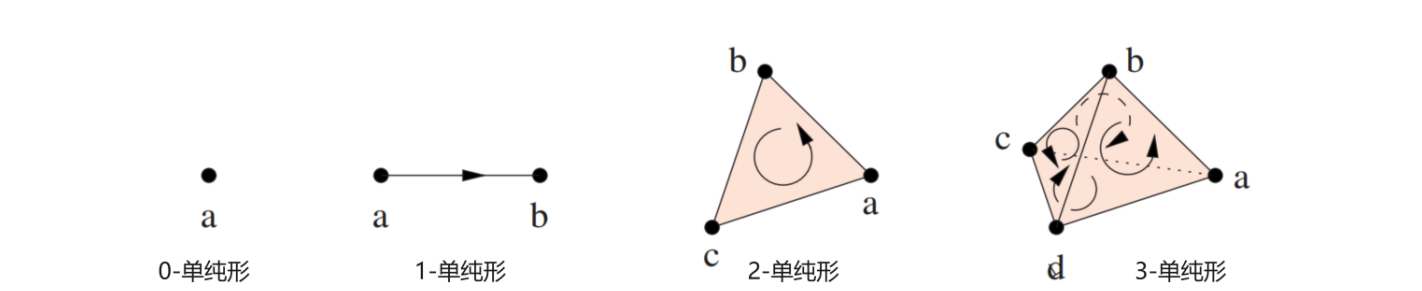
\includegraphics[width=1.1\textwidth]{figure/单纯形.png}
    \caption{不同维度单形示意图}
\end{figure}

\textbf{定义 2.9} (单纯复形)\cite{zomorodian2004computing}:
一个(几何)\textbf{单纯复形 (simplicial complex)} $K$ 是 $\mathbb{R}^m$ 中有限个单纯形的集合,并满足以下两个条件:
\begin{enumerate}
    \item 如果一个单纯形 $\sigma \in K$,那么 $\sigma$ 的所有面也都属于 $K$。
    \item 如果 $K$ 中任意两个单纯形 $\sigma_1, \sigma_2 \in K$ 的交集 $\sigma_1 \cap \sigma_2$ 非空,那么这个交集必须是 $\sigma_1$ 的一个面,并且也是 $\sigma_2$ 的一个面。
\end{enumerate}
单纯复形的 \textbf{维度 (dimension)} 是其包含的所有单纯形中的最大维度。

单纯复形为我们提供了一种将离散点云数据组合成具有拓扑结构的连续对象(的近似)的方法。通过研究单纯复形的拓扑性质(如连通分支、环、空腔等),我们可以了解原始数据的“形状”。在持续同调的计算中,通常会构建一系列嵌套的单纯复形(即过滤,详见下一小节),以分析拓扑特征在不同尺度下的演化。
\begin{figure}[thbp!]
    \centering
    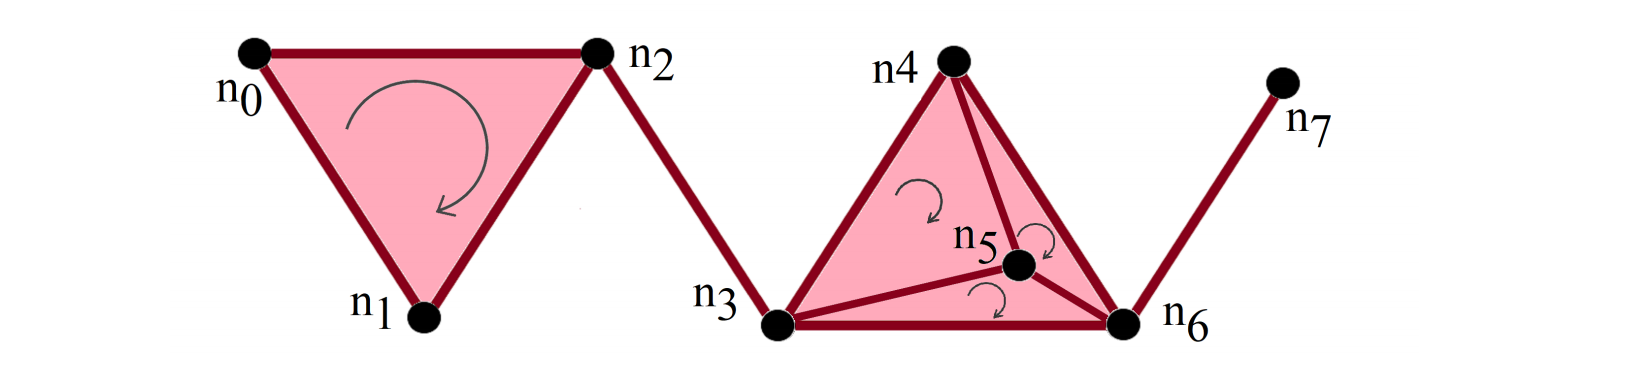
\includegraphics[width=.9\textwidth]{figure/单形集合.png}
    \caption{单纯复形示意图}
\end{figure}
\subsubsection{过滤}
% 这里补充定义
在定义了单纯复形之后,为了能够分析数据在不同尺度下的拓扑特征如何演化,我们需要引入过滤的概念。过滤为持续同调的计算提供了基础,它允许我们追踪拓扑特征(如连通分支、环等)的“生命周期”。

\textbf{定义 2.10} (过滤):
一个单纯复形 $K$ 的 \textbf{过滤 (filtration)} 是指 $K$ 的一系列嵌套子复形(subcomplexes)的序列:
$$ \emptyset = K_0 \subseteq K_1 \subseteq K_2 \subseteq \dots \subseteq K_n = K $$
这个序列通常由一个实值参数(称为过滤参数或尺度参数)$\alpha \in \mathbb{R}$ 来索引,使得当 $\alpha_i \le \alpha_j$ 时,有 $K_{\alpha_i} \subseteq K_{\alpha_j}$。换句话说,随着过滤参数的增加,单纯复形通过不断加入新的单纯形而“增长”。

在实际应用中,过滤通常是从一个点云数据 $P$ 开始构建的。一个常见的构建过滤的方法是利用 Vietoris-Rips 复形(通常简称为 Rips 复形)。

\textbf{定义 2.11} (Vietoris-Rips 过滤)\cite{zomorodian2004computing}:
给定一个度量空间中的有限点云 $P = \{p_1, \ldots, p_N\}$ 和一个距离参数 $\epsilon \ge 0$。点云 $P$ 上的 \textbf{Vietoris-Rips 复形 (Vietoris-Rips complex)},记作 $\text{VR}(P, \epsilon)$(或 $R(P, \epsilon)$),是一个单纯复形,其顶点集为 $P$。一个由 $P$ 中的 $k+1$ 个顶点 $\{v_0, v_1, \ldots, v_k\}$ 构成的集合形成 $\text{VR}(P, \epsilon)$ 中的一个 $k$-单纯形,当且仅当这 $k+1$ 个顶点两两之间的距离都不超过 $\epsilon$,即对于所有的 $0 \le i < j \le k$,都有 $d(v_i, v_j) \le \epsilon$。

当距离参数 $\epsilon$ 从 $0$ 开始连续增大时,我们就得到了一系列的嵌套 Vietoris-Rips 复形:
$$ \text{VR}(P, \epsilon_0) \subseteq \text{VR}(P, \epsilon_1) \subseteq \dots \subseteq \text{VR}(P, \epsilon_m) $$
其中 $0 = \epsilon_0 < \epsilon_1 < \dots < \epsilon_m$ 是一系列离散的距离阈值。这个嵌套的复形序列就是一种 \textbf{Vietoris-Rips 过滤 (Vietoris-Rips filtration)}。

除了 Vietoris-Rips 过滤之外,Čech 复形是另一种从点云数据构建单纯复形的重要方法,它与开覆盖的神经(Nerve of an open cover)紧密相关,并具有良好的理论性质。

\textbf{定义 2.12} (Čech 复形)\cite{zomorodian2004computing}:
令 $(X, d)$ 为一个度量空间,其中 $X$ 是一个(通常为有限的)点集。对于给定的参数 $\varepsilon > 0$,令 $B(x, \varepsilon)$ 表示以点 $x \in X$ 为球心、$\varepsilon$ 为半径的闭球。考虑由这些球构成的集合 $\mathcal{B}_{\varepsilon}(X) = \{B(x, \varepsilon) \mid x \in X\}$,这是一个对 $X$ 中各点邻域的覆盖(尽管它本身可能不是对某个更大空间的完整覆盖)。
这个覆盖 $\mathcal{B}_{\varepsilon}(X)$ 的 \textbf{神经 (Nerve)},记为 $N(\mathcal{B}_{\varepsilon}(X))$,即为点集 $X$ 上参数为 $\varepsilon$ 的 \textbf{Čech 复形 (Čech complex)},记作 $C(X, \varepsilon)$。其定义如下:
$C(X, \varepsilon)$ 的顶点集为点集 $X$ 本身。一个由 $X$ 中的 $k+1$ 个顶点组成的集合 $\{\alpha_0, \alpha_1, \ldots, \alpha_k\}$ 构成 $C(X, \varepsilon)$ 中的一个 $k$-单纯形(记作 $\langle \alpha_0, \alpha_1, \ldots, \alpha_k \rangle$),当且仅当这些顶点对应的半径为 $\varepsilon$ 的闭球的交集非空,即:
$$ \bigcap_{j=0}^{k} B(\alpha_j, \varepsilon) \neq \emptyset $$
其中 $\alpha_j \in X$, $0 \le j \le k$。

与 Vietoris-Rips 复形类似,当参数 $\varepsilon$ 从 $0$ 开始增加时,Čech 复形也形成一个嵌套序列 $C(X, \varepsilon_0) \subseteq C(X, \varepsilon_1) \subseteq \dots \subseteq C(X, \varepsilon_m)$,构成一个 \textbf{Čech 过滤 (Čech filtration)}。根据神经定理 (Nerve Theorem),在一定条件下,Čech 复形的同调群能够准确地反映其覆盖球并集的同调群,这使其在理论分析中具有重要地位。然而,由于判断多个球交集是否非空的计算复杂度较高,实际应用中 Vietoris-Rips 复形更为常见。
% 插入图片
\begin{figure}[thbp!]
    \centering
    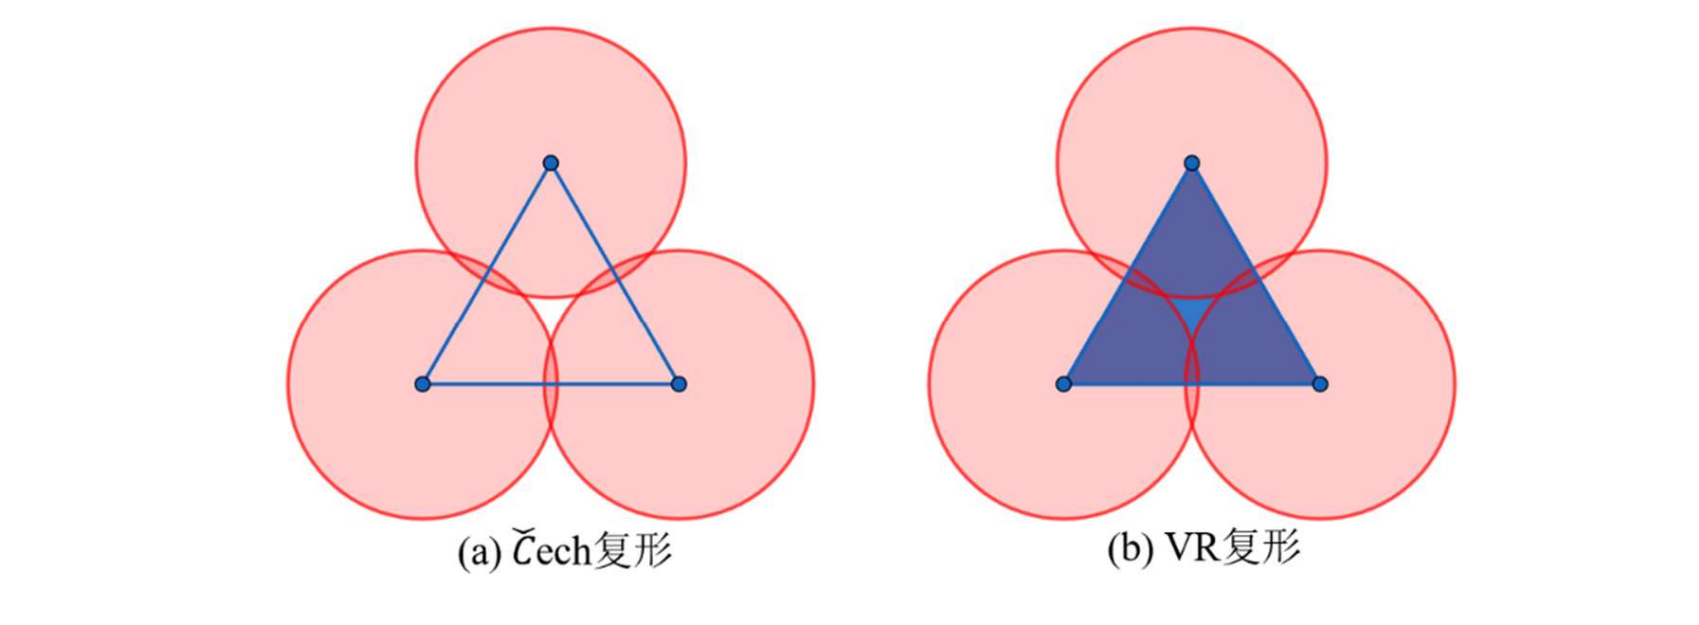
\includegraphics[width=.9\textwidth]{figure/VR复形.png}
    \caption{Čech 复形与 VR 复形}
\end{figure}
过滤的概念是至关重要的,因为它将静态的几何结构(点云)与动态的拓扑演化联系起来。通过分析在过滤过程中拓扑特征如何出现(出生)和消失(死亡),持续同调能够量化这些特征的“持续性”,从而区分数据中显著的结构和可能由噪声引起的短暂结构。Zomorodian(2005)\cite{zomorodian2004computing} 的工作正是提供了计算这种过滤复形序列的持续同调的有效算法。
\subsubsection{同调群与贝蒂数}
% 这里补充定义
为了从单纯复形中定量地描述其拓扑特征(如连通分支、环、空腔等),代数拓扑学引入了同调群的概念。同调群的构建始于链群和边缘算子。

\textbf{定义 2.13} (链群)\cite{armstrong2013basic}:
设 $K$ 是一个有限单纯复形。对于一个非负整数 $q$, $K$ 的 $q$ 维 \textbf{链 (chain)} 是 $K$ 中所有(赋固定系数环/域 $G$ 中元素的)定向 $q$-单纯形的形式线性组合。所有 $q$ 维链在系数的加法运算下构成一个阿贝尔群(当 $G$ 是域时,构成一个向量空间),称为 $K$ 的 $q$ 维 \textbf{链群 (chain group)},记作 $C_q(K; G)$ 或简记为 $C_q(K)$(当系数环/域 $G$ 从上下文中明确时,如常取整数环 $\mathbb{Z}$ 或二元域 $\mathbb{Z}_2$)。
具体地,若 $\sigma_1, \sigma_2, \ldots, \sigma_m$ 是 $K$ 中所有的(已选定方向的) $q$-单纯形,则 $C_q(K; G)$ 中的任一元素(即 $q$-链)可表示为 $c = \sum_{i=1}^m g_i \sigma_i$,其中系数 $g_i \in G$。

\textbf{定义 2.14} (边缘算子、闭链群与边缘链群)\cite{armstrong2013basic}:
对于每个维度 $q \ge 0$,存在一个称为 \textbf{边缘算子 (boundary operator)} 的同态映射 $\partial_q: C_q(K) \to C_{q-1}(K)$。它将一个 $q$-单纯形 $\sigma = \langle v_0, v_1, \ldots, v_q \rangle$ 映射到其所有 $(q-1)$-维面的(带适当定向和系数的)和,通常定义为 $\partial_q \sigma = \sum_{j=0}^q (-1)^j \langle v_0, \ldots, \hat{v}_j, \ldots, v_q \rangle$,其中 $\hat{v}_j$ 表示去掉顶点 $v_j$。对于 $q=0$,定义 $\partial_0 = 0$。边缘算子具有核心性质 $\partial_{q-1} \circ \partial_q = 0$(即 $\partial^2 = 0$)对所有 $q \ge 1$ 成立。

边缘算子 $\partial_q: C_q(K) \to C_{q-1}(K)$ 的 \textbf{核 (kernel)},即满足 $\partial_q c = 0$ 的所有 $q$-链 $c \in C_q(K)$ 的集合,称为 $K$ 的 $q$ 维 \textbf{闭链群 (group of $q$-cycles)},记作 $Z_q(K)$。$Z_q(K)$ 中的元素称为 $q$ 维 \textbf{闭链 (cycle)},它们是没有代数边界的 $q$-链。

边缘算子 $\partial_{q+1}: C_{q+1}(K) \to C_q(K)$ 的 \textbf{像 (image)},即所有形如 $\partial_{q+1} d$(其中 $d \in C_{q+1}(K)$)的 $q$-链的集合,称为 $K$ 的 $q$ 维 \textbf{边缘链群 (group of $q$-boundaries)},记作 $B_q(K)$。$B_q(K)$ 中的元素称为 $q$ 维 \textbf{边缘链 (boundary)},它们是 $(q+1)$-链的边界。
由 $\partial_q \circ \partial_{q+1} = 0$ 可知,$B_q(K)$ 是 $Z_q(K)$ 的一个子群,即 $B_q(K) \subseteq Z_q(K)$。

\textbf{定义 2.15} (同调群)\cite{armstrong2013basic}:
令 $K$ 为一个单纯复形,$Z_q(K)$ 和 $B_q(K)$ 分别为复形 $K$ 的 $q$ 维闭链群和 $q$ 维边缘链群。它们的商群
$$ H_q(K) = Z_q(K) / B_q(K) $$
称为 $K$ 的(基于所选系数的) $q$ 维 \textbf{同调群 (homology group)}。

同调群 $H_q(K)$ 的元素是闭链在模去边缘链意义下的等价类。直观上,同调群捕捉了那些不能被“填充”为更高维对象边界的 $q$ 维“孔洞”。在同调群的计算中,通过对边缘链群取商可以剔除边界的影响,从而更加准确地描述拓扑空间的内部结构。通过对复形的同调群计算,可以提取数据的拓扑不变量,进而从中分析相同类别的点云中存在的统一拓扑结构。然而,形成于同一类别时间数据的 Rips 复形并不一定能够在某个距离参数 $\varepsilon$ 下具有相同的同调群,因此需要采取更好的方法来分析数据的拓扑特征。持久同调方法可以通过计算不同距离参数下的单纯复形序列的同调,来逼近原始数据集的拓扑结构。

\textbf{定义 2.16} (贝蒂数)\cite{armstrong2013basic}:
单纯复形 $K$ 的 $q$ 维同调群 $H_q(K; G)$(当系数 $G$ 为一个域时,它是一个向量空间)的 \textbf{秩 (rank)}(或维度),称为 $K$ 的第 $q$ 个 \textbf{贝蒂数 (Betti number)},用 $\beta_q(K)$ 或简记为 $\beta_q$ 表示。它等于 $q$ 维闭链群的秩减去 $q$ 维边缘链群的秩,即:
$$ \beta_q = \text{rank } H_q(K) = \text{rank } Z_q(K) - \text{rank } B_q(K) $$
(此处的秩理解为相应阿贝尔群的自由部分的秩,或者当以域为系数时理解为向量空间的维数。)
$q$ 维贝蒂数是拓扑空间的一种拓扑不变量,它用来衡量拓扑空间中 $q$ 维孔洞的数量。具体而言:$\beta_0$ 表示拓扑空间中连通分支的数量,$\beta_1$ 表示拓扑空间中独立“环”或一维孔洞的数量,而 $\beta_2$ 则表示拓扑空间中独立“空腔”或二维孔洞的数量。

\subsubsection{持续同调}
% 这里补充定义
在拓扑数据分析中,(标准的)同调群是一种用于描述单个拓扑空间中孔洞信息的代数工具。通过同调群可以揭示拓扑空间的内在性质,例如空间的连通分支数量、环的数量、空腔的数量等。然而,当处理通过过滤(filtration)得到的单纯复形序列时,我们更关心这些拓扑特征是如何随尺度参数的变化而持续存在的。

令 $K$ 是一个初始单纯复形,一个过滤是指由其子复形构成的一系列嵌套集合:
$$ \emptyset = K_0 \subseteq K_1 \subseteq K_2 \subseteq \dots \subseteq K_n = K $$
其中,每个包含关系 $K_i \subseteq K_{i+1}$ 都是一个单纯映射,这个映射会在它们各自的同调群之间诱导一个同态 $f_{i, i+1}^q: H_q(K_i) \to H_q(K_{i+1})$(对于每个维度 $q$)。这一系列的同调群和由包含映射诱导的同态构成了一个 \textbf{持续模 (persistence module)}。持续同调正是研究这些持续模的代数结构,以追踪在过滤过程中拓扑特征的“出生”(出现)与“死亡”(消失)。

\textbf{定义 2.17} (持续同调群):
考虑一个由参数 $\varepsilon \ge 0$ 索引的过滤复形序列 $F = \{K^\varepsilon \mid \varepsilon \ge 0\}$,其中当 $\varepsilon_i \le \varepsilon_j$ 时,有 $K^{\varepsilon_i} \subseteq K^{\varepsilon_j}$。对于任意 $\varepsilon_i \le \varepsilon_j$,由包含映射 $K^{\varepsilon_i} \hookrightarrow K^{\varepsilon_j}$ 诱导的 $q$ 维同调群之间的同态记为 $f_q^{\varepsilon_i, \varepsilon_j}: H_q(K^{\varepsilon_i}) \to H_q(K^{\varepsilon_j})$。
在参数值从 $\varepsilon_i$ 增加到 $\varepsilon_j$ 的过程中,那些在 $H_q(K^{\varepsilon_i})$ 中出现并且通过 $f_q^{\varepsilon_i, \varepsilon_j}$ 映射到 $H_q(K^{\varepsilon_j})$ 中非平凡元素的同调类,被认为是“持续存在的”。更精确地,第 $q$ 维的 $(\varepsilon_i, \varepsilon_j)$-\textbf{持续同调群 (persistent homology group)} 定义为诱导同态 $f_q^{\varepsilon_i, \varepsilon_j}$ 的像(image):
$$ H_q^{\varepsilon_i, \varepsilon_j} = \text{im}(f_q^{\varepsilon_i, \varepsilon_j}) = f_q^{\varepsilon_i, \varepsilon_j}(H_q(K^{\varepsilon_i})) $$
$H_q^{\varepsilon_i, \varepsilon_j}$ 的秩(或维度,当以域为系数时)即为在尺度区间 $[\varepsilon_i, \varepsilon_j)$ 内持续存在的 $q$ 维拓扑特征的数量。

持续同调方法的核心优势在于其能够量化过滤流 $F$ 中拓扑特征随参数半径(或其他过滤参数)变化的动态过程。随着参数半径的增加,原有的复形结构会通过添加新的单纯形而增长,这会导致新的孔洞结构产生,而已有的孔洞也可能因为更高维单纯形的加入而被“填充”从而消失。为了系统地分析这些孔洞的出生 (birth) 和消亡 (death) 信息,并提取稳定的拓扑特征,研究者们发展了多种方法,其中最常用的是将持续同调的结果总结为持续图(persistence diagram)。

\subsection{从点云构建复形过滤}
将时间序列数据转换为高维欧几里得空间 $\mathbb{R}^d$ 中的点云 $P$ 是进行拓扑数据分析的前置步骤。然而,点云本身仅为离散点的集合,缺乏描述点与点之间连接关系或更高维度结构(如环、空腔)的内在信息。拓扑数据分析,特别是持续同调(Persistent Homology, PH),正是通过分析点云数据所隐含的这种高阶结构来量化数据的“形状”特征。至关重要的是,持续同调并非直接作用于原始点云,而是作用于从点云数据构建的单纯复形(Simplicial Complex)或类似组合结构(如立方复形)之上。更进一步,持续同调的核心在于研究拓扑特征如何在不同尺度(scale)下演化并持续存在。因此,仅仅构建单个复形是不够的,必须构建一个随尺度参数变化的复形序列,即所谓的过滤(Filtration)。这一过程是连接点云的几何表示与持续同调所揭示的拓扑不变量之间的关键桥梁。

从点云 $P \subset \mathbb{R}^d$ 构建单纯复形的基本思想是基于点的“邻近性”:若一组点在某种意义上彼此足够接近,则它们应共同构成一个结构单元(即单形)。这种邻近度通常由一个非负的尺度参数 $\epsilon$ 来量化。随着 $\epsilon$ 的增加,越来越多的点集被认为是“邻近”的,从而允许形成更高维度的单形,使得复形的整体结构逐渐丰富和复杂化。这种随 $\epsilon$ 增长而形成的、在集合包含关系上单调递增的复形序列 $K_{\epsilon_0} \subset K_{\epsilon_1} \subset \dots \subset K_{\epsilon_n}$(其中 $0 \le \epsilon_0 < \epsilon_1 < \dots < \epsilon_n$)即构成了过滤流,这是计算持续同调的标准输入。

\subsubsection{Vietoris-Rips复形实例}
在信号分析的拓扑方法中,一个核心步骤是从时间序列数据生成点云,并进一步构造单纯复形以揭示其潜在的几何与拓扑特性。这里关注Perea等人\cite{perea2015sliding}运用的滑动窗口嵌入(Sliding Window Embedding)技术以及由此产生的点云所构建的Rips复形。

首先,介绍滑动窗口嵌入方法。假设有一个在实数区间上定义的函数 $f$(例如,一个时间序列信号)。选择一个正整数 $M$ 和一个正实数 $\tau$(时间延迟)。在时间点 $t \in \mathbb{R}$,函数 $f$ 到 $\mathbb{R}^{M+1}$ 维空间的滑动窗口嵌入点 $SW_{M,\tau}f(t)$ 定义为:
\begin{equation}
    SW_{M,\tau}f(t) = \begin{bmatrix} f(t) \\ f(t+\tau) \\ \vdots \\ f(t+M\tau) \end{bmatrix}
\end{equation}
通过在不同的时间点 $t$ 上进行采样,可以得到一个点云集合,即滑动窗口点云(Sliding Window Point Cloud)。这个点云是后续拓扑分析的基础。此嵌入的一个关键参数是窗口大小(window-size)$M\tau$。

获得了滑动窗口点云 $X$(通常是一个紧致集,例如由有限个采样点构成)后,采用Rips复形进行构造。给定一个距离参数 $r \ge 0$,点云 $X$ 上的Rips复形,记作 $R_r(X)$,是一个单纯复形,其顶点集即为点云 $X$ 中的点。一个包含 $k+1$ 个顶点 $\{x_0, x_1, \ldots, x_k\}$ 的集合构成 $R_r(X)$ 中的一个 $k$-单纯形(记作 $[x_0, x_1, \ldots, x_k]$),当且仅当该集合中任意两个不同顶点 $x_i, x_j$ 之间的欧氏距离(或其他定义好的度量)满足以下条件:
\begin{equation}
    \|x_i - x_j\| \leq r \quad \forall 0 \leq i < j \leq k
\end{equation}
值得注意的是,Rips复形的构造仅依赖于其一维骨架(即边):一个高维单纯形被包含在复形中,当且仅当它的所有边(即所有顶点对)都满足上述距离条件。通过改变参数 $r$ 的值,可以得到一个嵌套的复形序列 $R_0(X) \subset R_{r_1}(X) \subset \ldots \subset R_{r_m}(X)$,这构成了Rips过滤(Rips filtration),是计算持久同调的基础。

这种从信号到点云再到过滤复形的过程,使得可以运用持久同调来量化信号的周期性等特征。


\subsubsection{witness复形实例}
当点云 $P$ 的规模非常大时,构建VR复形的计算开销会非常高。为了解决这个问题,可以使用 Witness 复形\cite{de2004topological}。Witness 复形是在点云 $P$ 的一个(通常较小的)子集 $Q = \{q_1, q_2, \ldots, q_M\} \subset P$ (称为地标点,landmark points) 上构建的,但其结构依然受到整个点云 $P$ (称为 witness 点) 的影响。地标点可以通过最大最小采样 (maxmin) 或随机采样等方法从 $P$ 中选取。Mittal\cite{mittal2017topological}论文中提到了两种类型的Witness复形,其定义基于“被见证”的概念:

一个由地标点构成的单纯形 $\sigma = [q_{j_0}, q_{j_1}, \ldots, q_{j_k}]$ (其中 $q_{j_l} \in Q$) 被点云 $P$ 中的一个点 $x \in P$ (称为 witness) 所“弱见证”(weakly witnessed),若对于 $\sigma$ 中的每一个顶点 $q \in \{q_{j_0}, \ldots, q_{j_k}\}$ 以及任意一个不在 $\sigma$ 中的地标点 $p \in Q \setminus \{q_{j_0}, \ldots, q_{j_k}\}$,都满足以下距离关系:
\begin{equation}
    d(q, x) \le d(p, x)
\end{equation}
这个条件意味着,相对于 witness 点 $x$ 而言,单纯形 $\sigma$ 中的所有顶点 $q$ 比任何不在 $\sigma$ 中的地标点 $p$ 都更近(或等近)。

基于此,弱 Witness 复形 $\mathcal{W}_{weak}(P, Q)$ 定义为包含所有那些能够被点云 $P$ 中至少一个点 $x \in P$ 所弱见证的地标单纯形 $\sigma \subseteq Q$ 的集合。

进一步地,强 Witness 复形 $\mathcal{W}_{strong}(P, Q)$ 对见证条件有更严格的要求。一个地标单纯形 $\sigma = [q_{j_0}, \ldots, q_{j_k}]$ 属于强 Witness 复形,如果它被某个 $x \in P$ 所弱见证,并且对于这个 $x$,它到 $\sigma$ 的所有顶点的距离都相等:
\begin{equation}
    d(q_{j_0}, x) = d(q_{j_1}, x) = \ldots = d(q_{j_k}, x)
\end{equation}
这两种Witness复形的构造都依赖于地标点和原始点云中 witness 点之间的距离关系,从而在降低计算复杂度的同时,试图捕捉原始点云的拓扑特征。

通过改变VR复形的尺度参数 $\epsilon$ 或Witness复形的选取方式(例如,地标点的数量或特定的见证半径,尽管本论文的定义更侧重相对距离),可以构建一个过滤的单纯复形序列,这是进行持久同调分析的基础。
